\documentclass[conference]{IEEEtran}
\IEEEoverridecommandlockouts
% The preceding line is only needed to identify funding in the first footnote. If that is unneeded, please comment it out.
\usepackage{cite}
\usepackage{amsmath,amssymb,amsfonts}
\usepackage{algorithmic}
\usepackage{graphicx}
\usepackage{textcomp}
\usepackage{xcolor}
\usepackage{derivative}
\def\BibTeX{{\rm B\kern-.05em{\sc i\kern-.025em b}\kern-.08em
    T\kern-.1667em\lower.7ex\hbox{E}\kern-.125emX}}
\begin{document}

\title{Effect of Injection and Valve Timing on Combustion Characteristics and Performance of Port-Fuelled Hydrogen Internal Combustion Engines
}

\author{\IEEEauthorblockN{I.M. Wickramaarachchi}
\IEEEauthorblockA{\textit{Department of Mechanical Engineering} \\
\textit{University of Moratuwa}\\
Katubedda, Sri Lanka \\
waisurumangala@gmail.com}
\and
\IEEEauthorblockN{J.S. Rassdeen}
\IEEEauthorblockA{\textit{Department of Mechanical Engineering} \\
\textit{University of Moratuwa}\\
Katubedda, Sri Lanka \\
waisurumangala@gmail.com}
\and
\IEEEauthorblockN{S. Kalana}
\IEEEauthorblockA{\textit{Department of Mechanical Engineering} \\
\textit{University of Moratuwa}\\
Katubedda, Sri Lanka \\
waisurumangala@gmail.com}
\and
\IEEEauthorblockN{N.A.I.D. Nissanka}
\IEEEauthorblockA{\textit{Department of Mechanical Engineering} \\
\textit{University of Moratuwa}\\
Katubedda, Sri Lanka \\
waisurumangala@gmail.com}
\and
\IEEEauthorblockN{Isuru Wickramaarachchi}
\IEEEauthorblockA{\textit{Department of Mechanical Engineering} \\
\textit{University of Moratuwa}\\
Katubedda, Sri Lanka \\
waisurumangala@gmail.com}
}

\maketitle

\begin{abstract}
The urgency of mitigating global warming has propelled hydrogen to the forefront as an alternative fuel.
However, abnormal combustion events pose a significant challenge in the development of Hydrogen Internal Combustion Engines (ICEs).
Adjustments of engine design parameters have demonstrated the possibility of controlling these issues.
Particularly, valve and injection timing are critical in mixture formation—a determinant of combustion behavior and engine performance.
Although previous research has primarily focused on the isolated effects of these parameters, their interdependence on each other is highly undeniable.
In this project, numerical simulations are carried out with detailed chemistry solver to comprehensively analyze the combined effect of valve and injection timing on the combustion characteristics and performance of port-fueled Hydrogen ICEs.
\end{abstract}

\begin{IEEEkeywords}
valve timing, injection timing, performance, combustion characteristics, hydrogen
\end{IEEEkeywords}

\section{Introduction}

Global warming presents the most severe environmental challenge today, primarily driven by the increased carbon dioxide (CO2) emissions from the consumption of fossil fuels.
The transportation sector, which heavily relies on ICEs, remains a major contributor to these emissions.
Consequently, the urgency to make these engines more sustainable and environmentally friendly is undeniable.
Efforts to address this issue led to the exploration and adoption of alternative fuels.
In this regard, hydrogen has emerged as a compelling option, taking advantage of its favourable combustion characteristics together with zero carbon emissions.\\

The literature identifies two distinct types of hydrogen ICEs: Port Fuel Injection (PFI) and Direct Injection (DI) engines.
PFI involves injecting fuel into the intake manifold, where it mixes with air before reaching the combustion chamber.
In contrast, DI engines inject hydrogen directly into the chamber during the compression stroke, initiating the ignition of the compressed air-fuel mixture.
Particularly, in DI engines, the processes of fuel-air mixing, and combustion occur simultaneously, leading to less time available for mixture formation.
To achieve sufficient mixing, higher injection pressures and precisely manufactured injectors are required, which leads to increased costs.
Conversely, PFI separates the mixing and combustion processes, affording more time for the creation of a uniform fuel-air mixture, eliminating the necessity for precisely manufactured injectors and the application of high injection pressures.
Therefore, PFI hydrogen engines represent a more viable solution for the rapid adaptation of alternative fuels.\\

Abnormal combustion including knocking and backfire are major problems found in hydrogen engines.
It has been demonstrated that those can be controlled by changing various design parameters including valve timing and injection timing.
Among the other parameters, valve and injection timing heavily affect the trapped hydrogen mass and mixture formation, which defines the combustion characteristics of ICEs.
The combustion process can lead to incomplete combustion or knocking combustion depending on the formed fuel-air mixture.\\

Although valve and injection timing are separately studied, their interdependency on each other is highly undeniable.
Both these parameters collectively define the mixture and thereby combustion characteristics and performance.
Therefore, a comprehensive understanding of the combined effect of valve and injection timing on combustion characteristics and performance is necessary to control injection timing and valve timing, in Hydrogen ICEs.\\

\section{Litreture Review}

Several studies showed the effect of valve and injection timing on combustion characteristics and performance.

\subsection{Injection Timing}

Wang \cite{b1} changed injection start times and monitored the hydrogen mass within the cylinder with crank angle.
The amount of trapped mass and mass backflow was different under each scenario.
The early injection caused less amount of backflow, and a higher fraction of mass could flow into the cylinder.
The backflow of hydrogen can be seen in every case after the compression stroke starts (after 540 CAD).
It can be explained using the push generated by the upward movement of the piston.
If the hydrogen injection is delayed, more hydrogen mass would be affected by this negative push, consequently reducing trapped hydrogen mass.
Yun \cite{b2} has measured the trapped hydrogen mass considering a wider range of injection timing.
In addition to the decreasing trend of trapped mass with delayed hydrogen injection, the effect of excessively early injection was also identified.
In combination, trapped hydrogen mass first increased and then decreased with the change of injection timing.
An optimum injection timing to trap the maximum amount of hydrogen mass could be observed.
Yun \cite{b2} also showed that the variation of indicated power and thermal efficiency was highly correlated with trapped hydrogen mass.
Therefore, to achieve higher engine performance, trapped hydrogen mass should be maximized.\\

Literature gives evidence of forming locally concentrated hydrogen mass near inlet valve seats due to improper injection timing.
Duan \cite{b3} showed that local concentration first increases and then decreases with injection delay.
When the injection is too early, hydrogen enters the inlet port and spreads towards the inlet valve before the valve opens.
When the injection is too late, hydrogen injection continuous after the intake valve closes, causing a high concentration mixture.
Liu \cite{b4} also showed this increasing trend of local concentration with excessively delayed injection timing.
In addition, excessively early or delayed injection also increases the maximum pressure in the intake port, following the same trend as the local concentration.
In the intermediate injection times, the pressure rise was minimal.
Backfire as an abnormal combustion phenomenon, usually characterized by increased intake manifold pressure.
Therefore, a comparison of the local concentration of hydrogen mass and intake manifold pressure implies that the local concentration of hydrogen near valve seats can strongly influence the backfiring risk.
Consequently, local hydrogen concentration can be used to identify the backfire possibility in port-fueled hydrogen engines.\\

\subsection{Valve Timing}

Menaa \cite{b5}, showed the variation of both trapped mass and backflow mass with the change of valve timing.
When the engine speed was lower than 2000 rpm, delaying Inlet Valve Close (IVC) caused a reduction in cylinder mass.
The behavior is the opposite with engine speeds higher than 2000 rpm.
With early IVC, backflow mass was insignificant compared to cylinder mass.
However, it is significant when the IVC is retarded.
Higher backflow mass leads to high local concentration near inlet valves, increasing the possibility of backfire.\\

Park \cite{b6} showed the effect of Inlet Valve Open (IVO) timing on engine performance and efficiency at the engine speed of 2000 rpm.
Torque had a decreasing trend with retarding IVO, while the efficiency first increased before decreasing.
This increase in thermal efficiency during the first half of the IVO delay was due to the decrease in trapped mass.
Huynh \cite{b7} studied a wider range valve overlap range from 00 - 500 to evaluate engine performance and showed that brake torque reduces in both low and excessive Valve Overlap Times (VOTs).
Reduction of engine performance was much more significant with low VOTs than with high VOTs.
VOT of 300 was shown to be the optimum VOT for the engine operating conditions in the study.
The study also showed that the probability of backfire decreases with a decrease in valve overlap.
The backfire limiting equivalence ratio, increased up to 1.2 with zero valve overlap.
This idea of backfire control by reducing VOT is also mentioned by Lee \cite{b8}.
The study conducted experiments to show that IVO timing can be used to control backfire with an ultra-lean mixture.
Results revealed that with a delay of 100CA, backfire-free operation can be ensured.\\

From these studies it is clear that valve timing affects both trapped mass and local hydrogen concentrations, consequently affecting combustion characteristics and engine performance.

\subsection{Research Gap}

Trapped hydrogen mass should be maximized to increase the performance of the engine while keeping the local concentrations near inlet valve seats at a minimum level to prevent backfire risks.
Although researchers have tried individual adjustments of valve and injection timing, it is their combined effect which defines both trapped mass and local concentration.
To control these parameters to improve engine performance while mitigating abnormal combustion events, a comprehensive understanding of their combined effect is necessary.

\section{Numerical Model}
\subsection{Governing Equations}
Reactive flow is governed by mass and momentum equations, energy equations, and species transport equations.

\subsubsection{Mass and momentum equations}

    \begin{gather*}
        \pdv{\rho}{t} + \pdv{(\rho u)}{ x} = 0
    \end{gather*}

    \begin{gather*}
        \pdv{(\rho u)}{t} + \pdv{(\rho uv)}{y} = - \pdv{p}{x} + \pdv{\tau\textsubscript{xy}}{y} + S\textsubscript{x}
    \end{gather*}

Where $\rho$ is density, $t$ is time, $u$, $v$ and $w$ are velocity component in $x$, $y$, and $z$ directions respectively. 
$p$ is pressure, $\tau\textsubscript{xy}$ is stress tensor, and $S\textsubscript{x}$ is the momentum source component.\\

\subsubsection{Energy equation}

    \begin{gather*}
        \pdv{(\rho e)}{t} + \pdv{(\rho ev)}{y} = -p \pdv{v}{y} + \tau \textsubscript{xy} \pdv{u}{y} + \pdv{(k \pdv{T}{y})}{y} + \pdv{(\rho D \sum h_m \pdv{Y_m}{y})}{y} + S
    \end{gather*}

Where $e$ is specific internal energy, $k$ is conductivity, $T$ is temperature, $D$ is coefficient of mass diffusion, $h_m$ is species enthalpy, $Y_m$ is mass fraction of species $m$ and $S$ is source term which accounts for energy sources.



\begin{table}[!ht]
    \centering
    \caption{Engine Specifications}
    \label{your_label_here}
    \begin{tabular}{|c|c|}
    \hline
    Header 1 & Header 2 \\
    \hline
    Bore & 92.6 mm \\
    Stroke & 86 mm \\
    Compression Ratio & 10.5 \\
    Equivalence Ratio & 0.59 \\
    Injection Duration & 155 CAD \\
    Engine Speed & 2000 RPM \\
    \hline
    \end{tabular}
    \end{table}

\section{Methodology}
\begin{itemize}
    \item Development of a validated numerical model.
    \item Analyze combustion characteristics with varying injection timing for the case of VOT = 300 to find suitable ranges of hydrogen injection.
    \item Evaluate combustion characteristics and performance for the range of valve and injection timing.
    \item Identify the combined effect of valve and injection timing on combustion characteristics and performance
\end{itemize}


\section{Numerical Model}
\subsection{Model Description}
Combustion models contain three regions including intake, cylinder, and exhaust. Redlich-Kwong gas equation is used for gas simulations. The Connaire reaction mechanism is used to calculate reaction rates. CFL number-based time stepping is used. The PISO algorithm is used for pressure velocity coupling. URANS-RNG k-epsilon model is used for turbulence modelling. O’Rourke and Amsden model are used to model wall heat transfer. For combustion modeling SAGE detailed chemistry solver is used. A high temperature energy source is used to model the ignition process while fuel injection is modelled as a mass inflow boundary condition.
\subsection{Mesh Sensitivity Analysis}
With the available computational power and license requirements, the maximum element count that we can run our simulations is 0.5 million. Mesh sensitivity analysis is carried out up to that point. The analysis shows that the mesh configuration with 8 mm base mesh is suitable for the analysis. The error compared to 6 mm base mesh configuration is only X percent.
\begin{figure}[htbp]
    \centerline{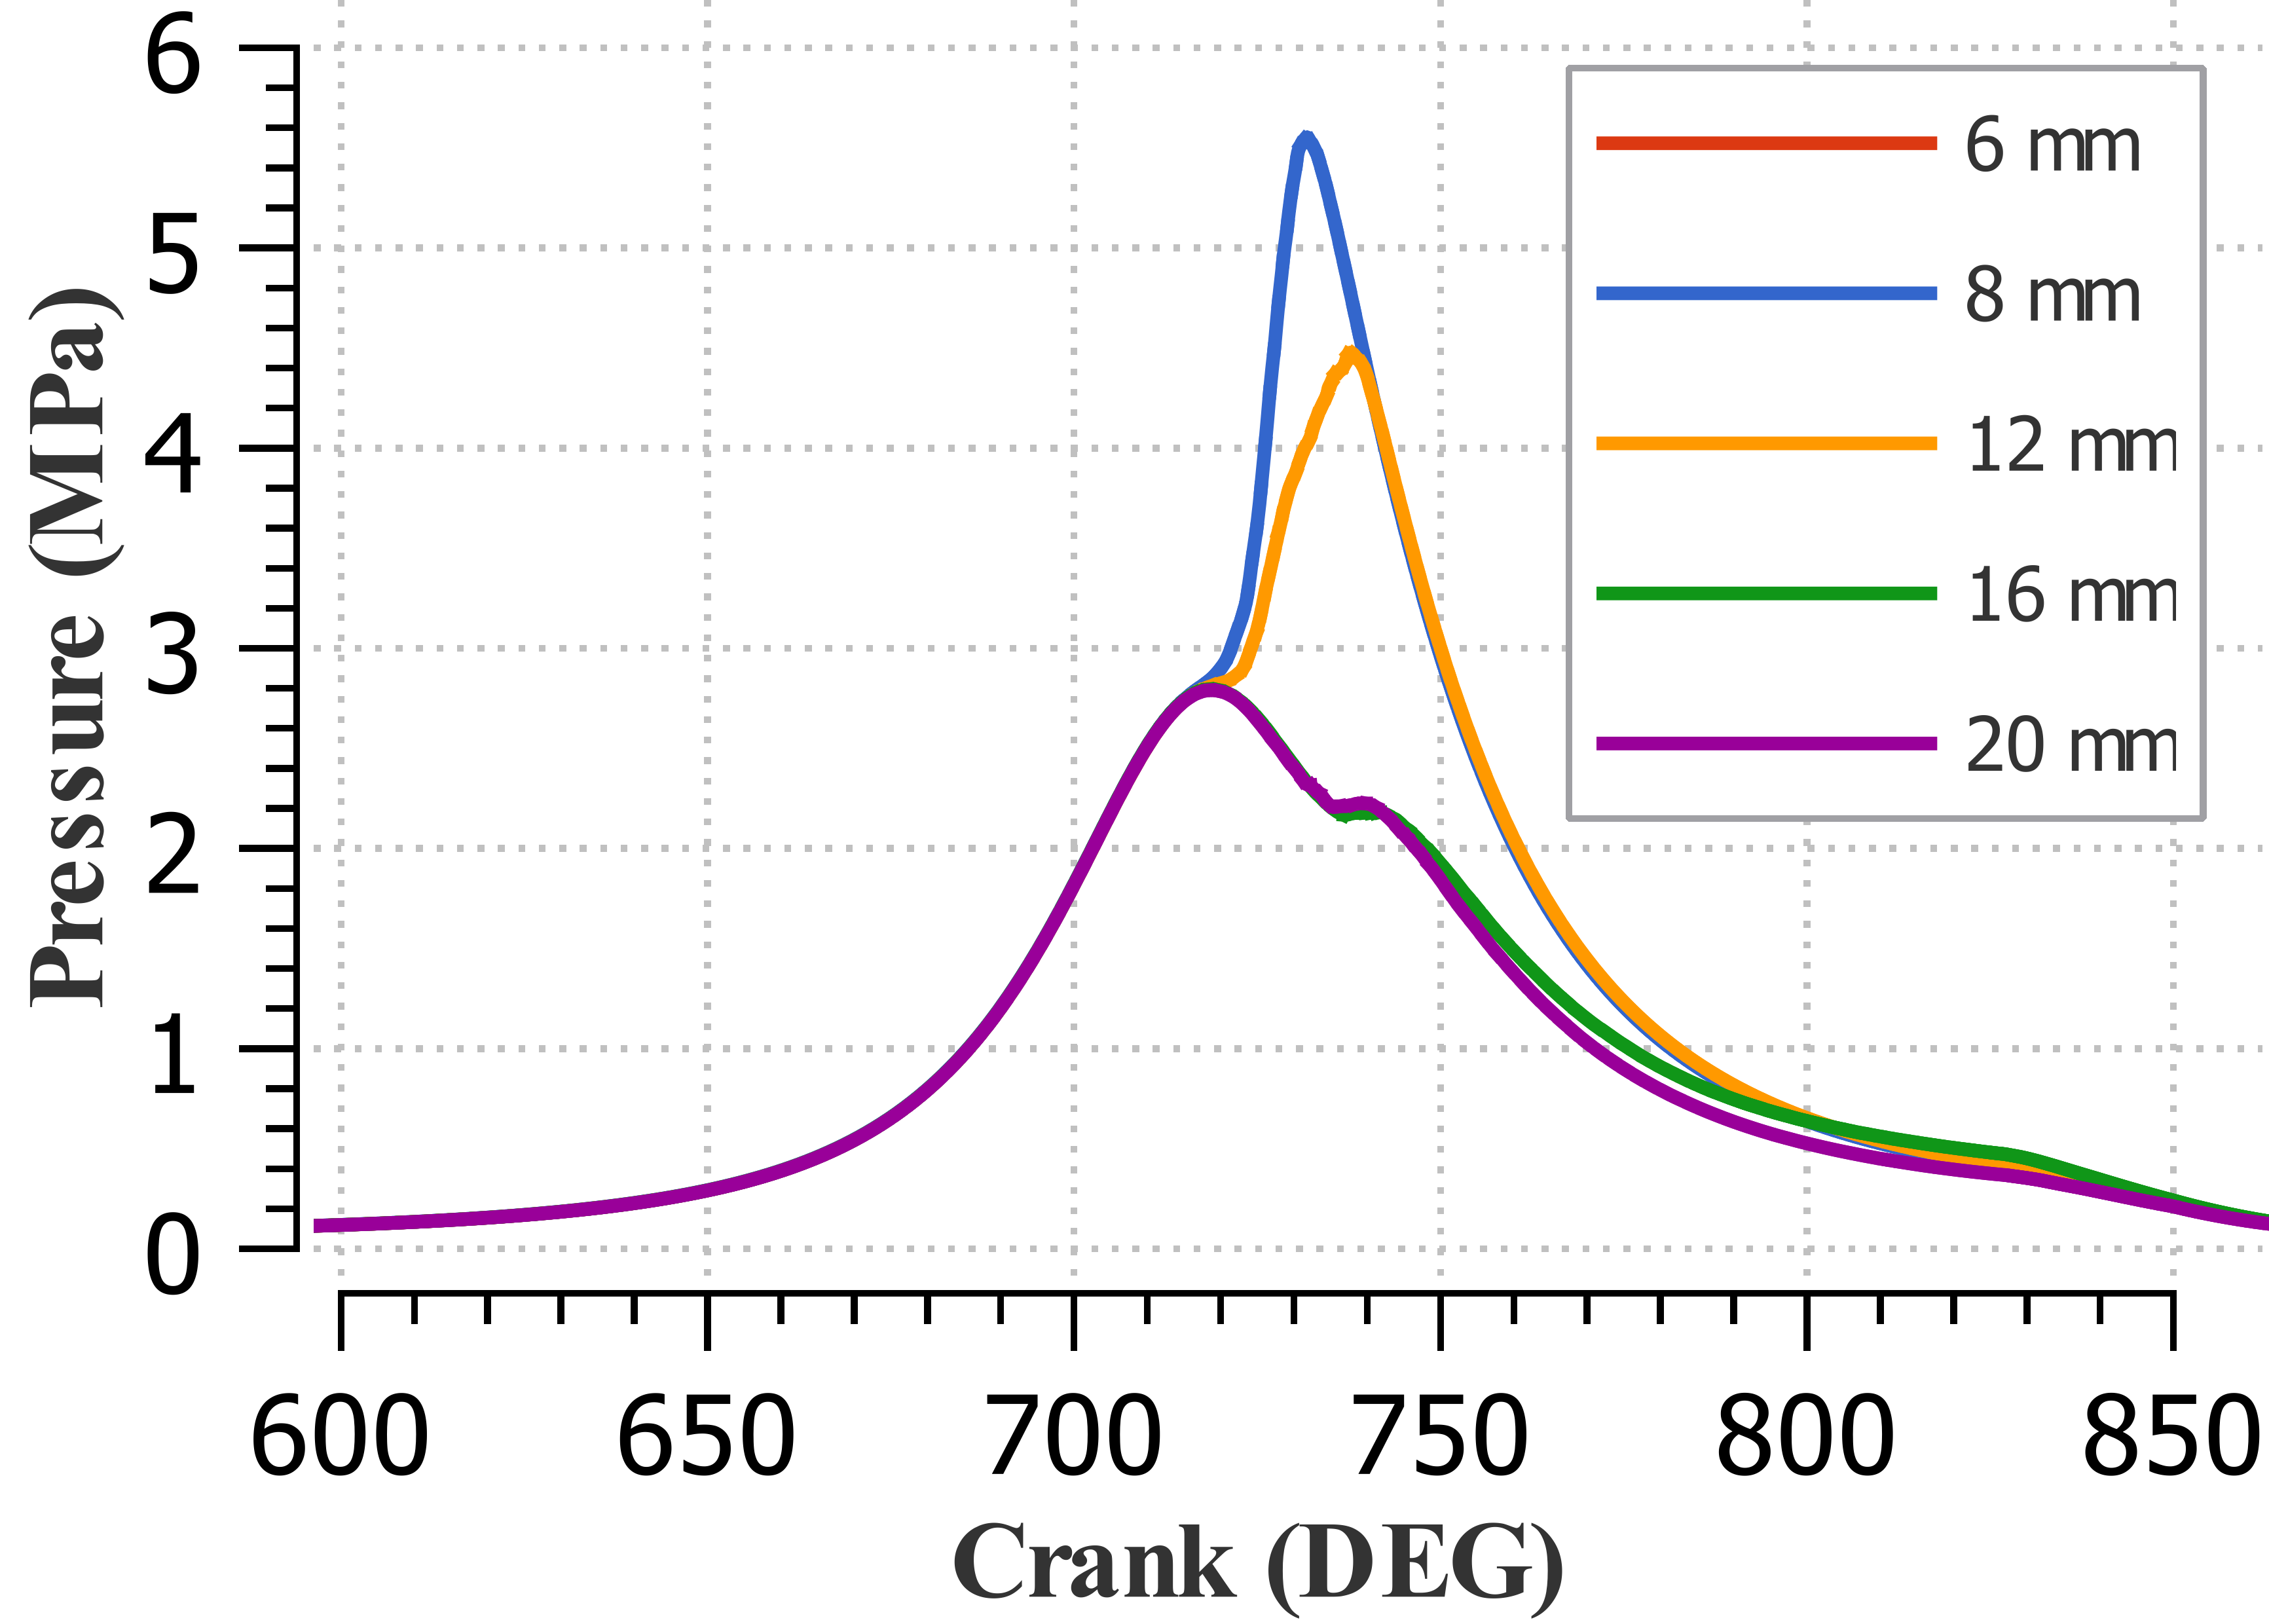
\includegraphics{Plots/mesh_sens.png}}
    \caption{Mesh Sensitivity}
    \label{plt_t}
    \end{figure}
\subsection{Model Validation}
As [4] also mentioned, simulation results are usually greater than experimental data due to limitations of computational mesh and from the fact that only one cylinder is modelled. Other than that, differences in the engine geometry also leads to deviation of results.
Although the maximum pressure differs by x percent, the numerical model follows the same trend as the experimental data. Therefore, this model can be used to find trends of the combustion process.

In the previous figure, we can see that the model is vlaidated.
    
\section{Analysis}
\subsection{Range Selection}
Valve overlap time range of 15-45 is selected for the analysis. reasons
VOT of 30 is first assumed to find the suitable range of injection timing with respect to intake valve open time, since VOT of 30 demonstrated the optimal engine performance in the study [7].
Range of start angles of 00 aIVO to 400 aIVO is tested for their combustion characteristics. 
It could be observed that, to properly combusts the mixture within the chamber while generating useful work injection start time of 200 aIVO to 300 aIVO is selected as possible range of injection.
Earlier injection leads knocking combustion while delayed injection leads to incomplete combustion.
Within the range injection start angles of 200 aIVO, 250 aIVO and 300 aIVO were selected as early, balanced, and delayed injection for all VOT values.

\begin{figure}[htbp]
    \centerline{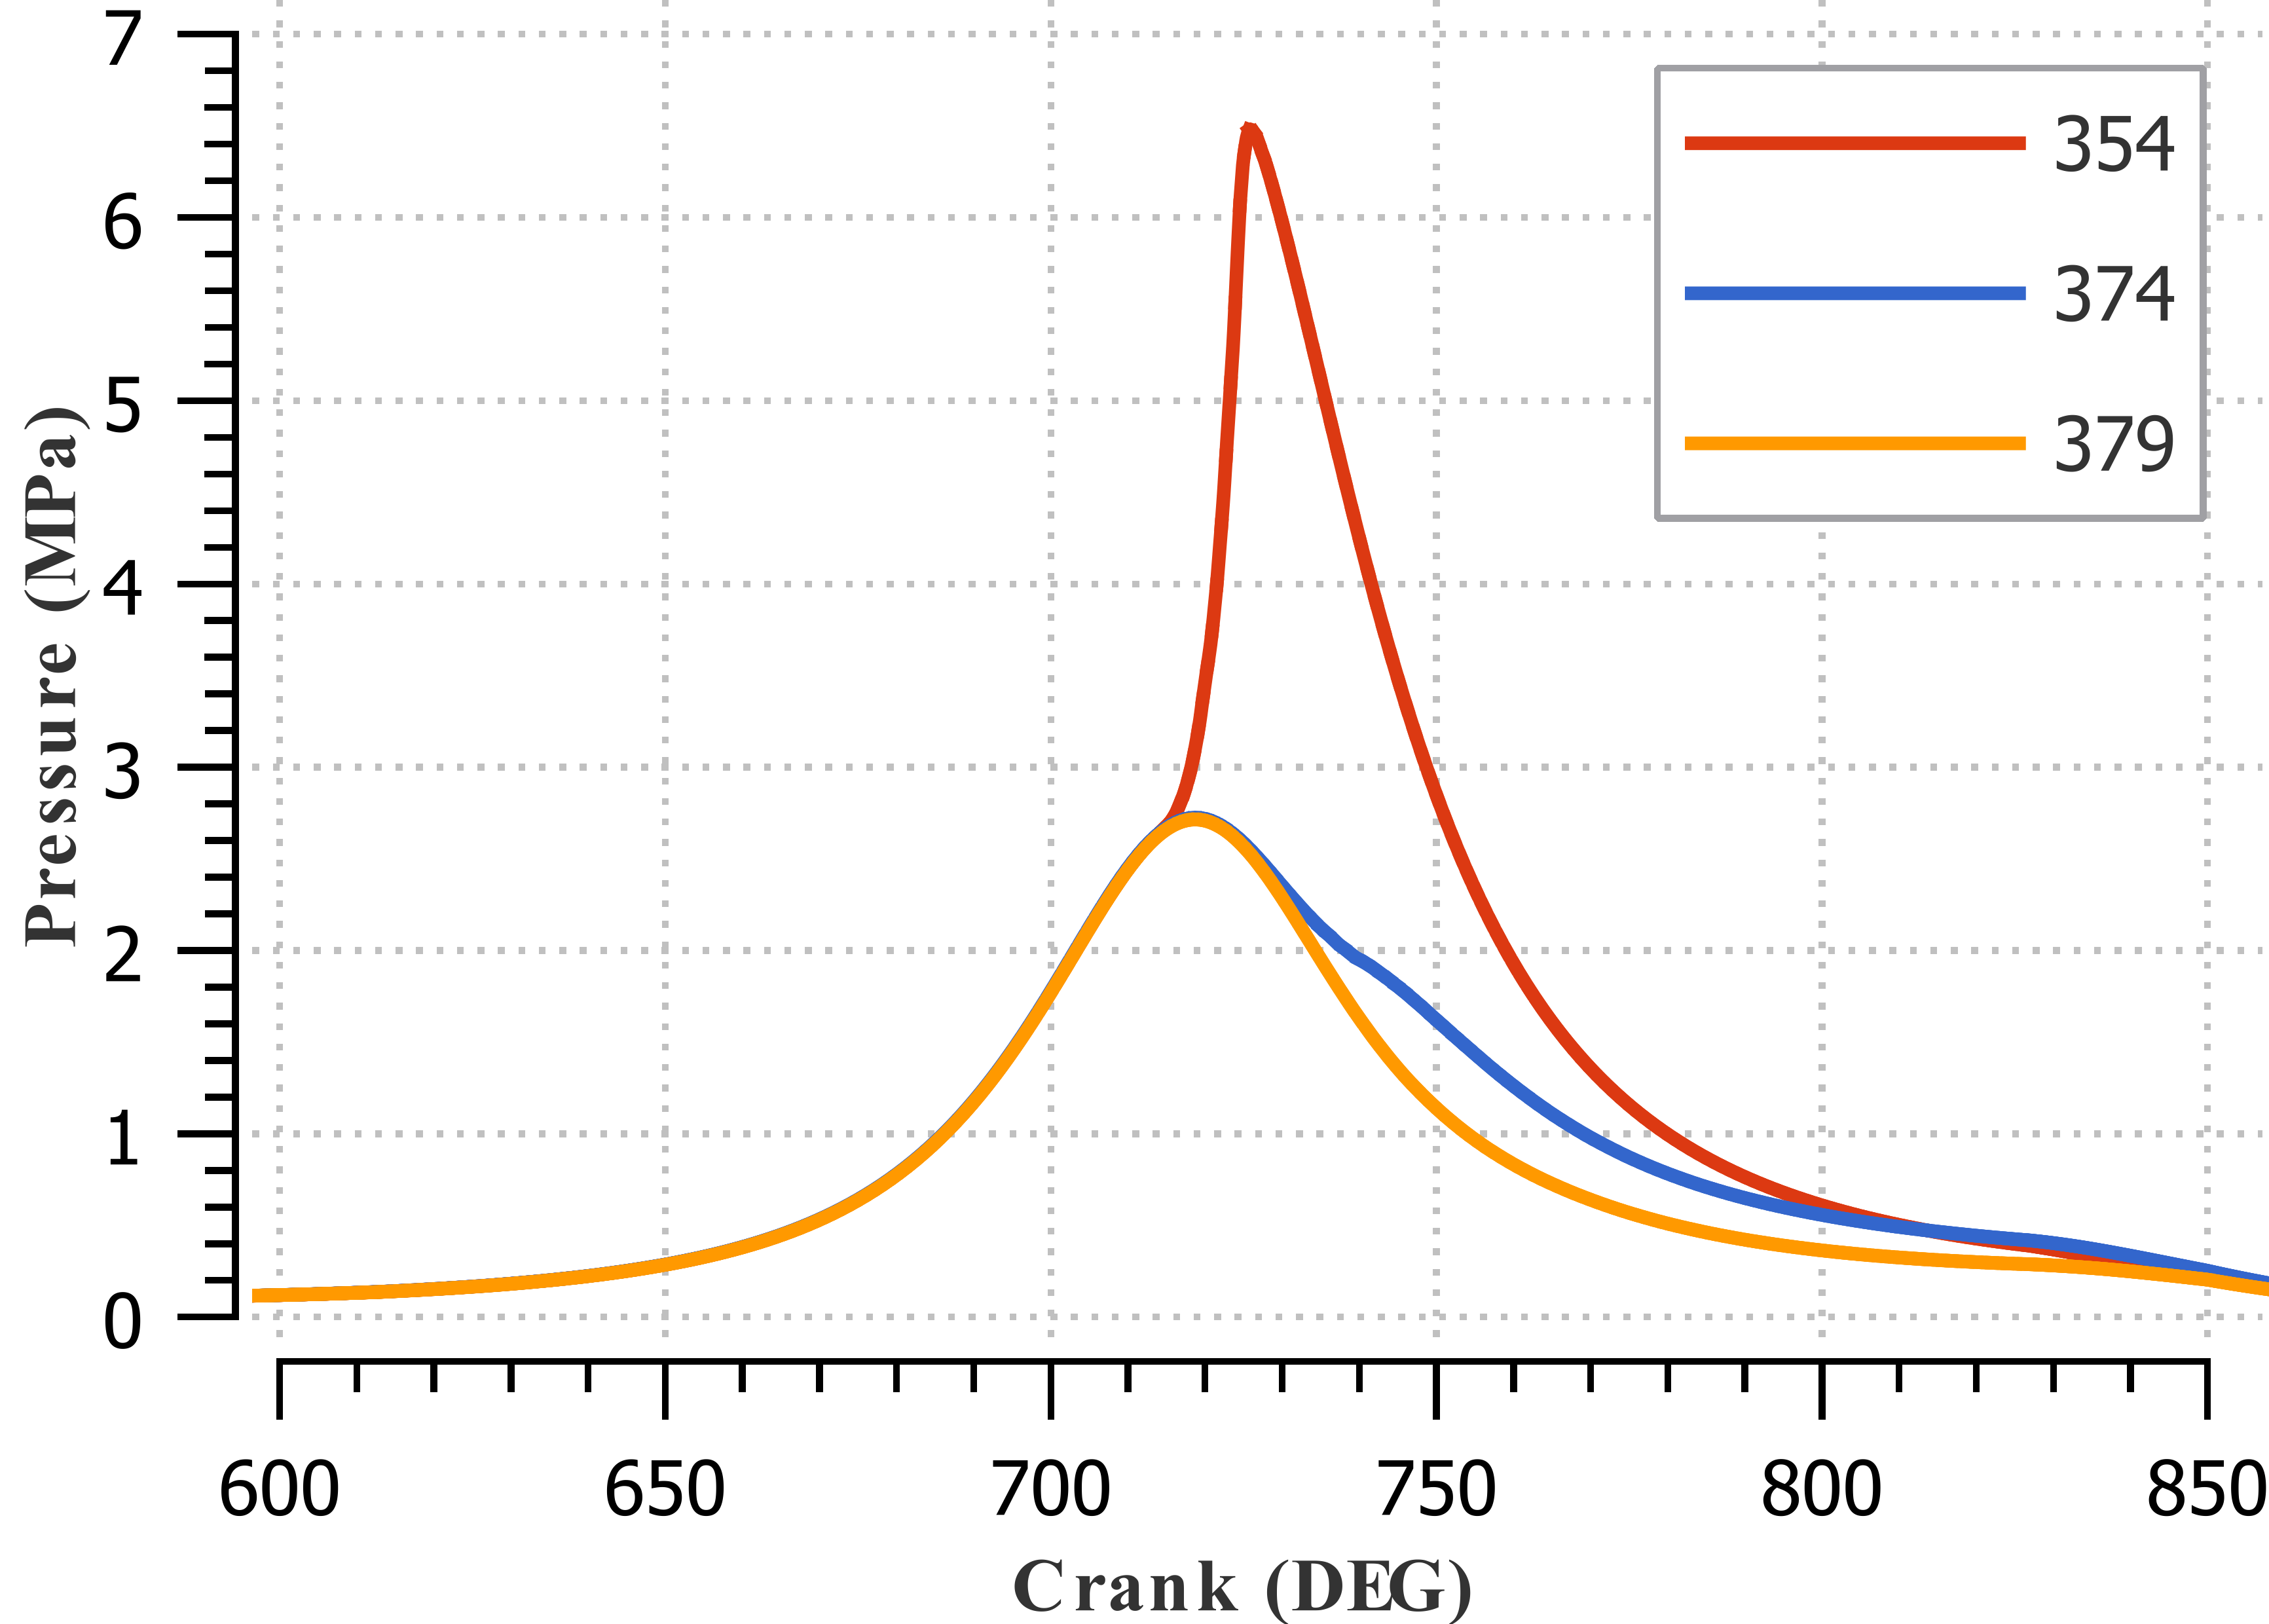
\includegraphics{Plots/30_pressure.png}}
    \caption{In-Cylinder Pressure for VOT = 30}
    \label{plt_tttt}
    \end{figure}

\begin{figure}[htbp]
    \centerline{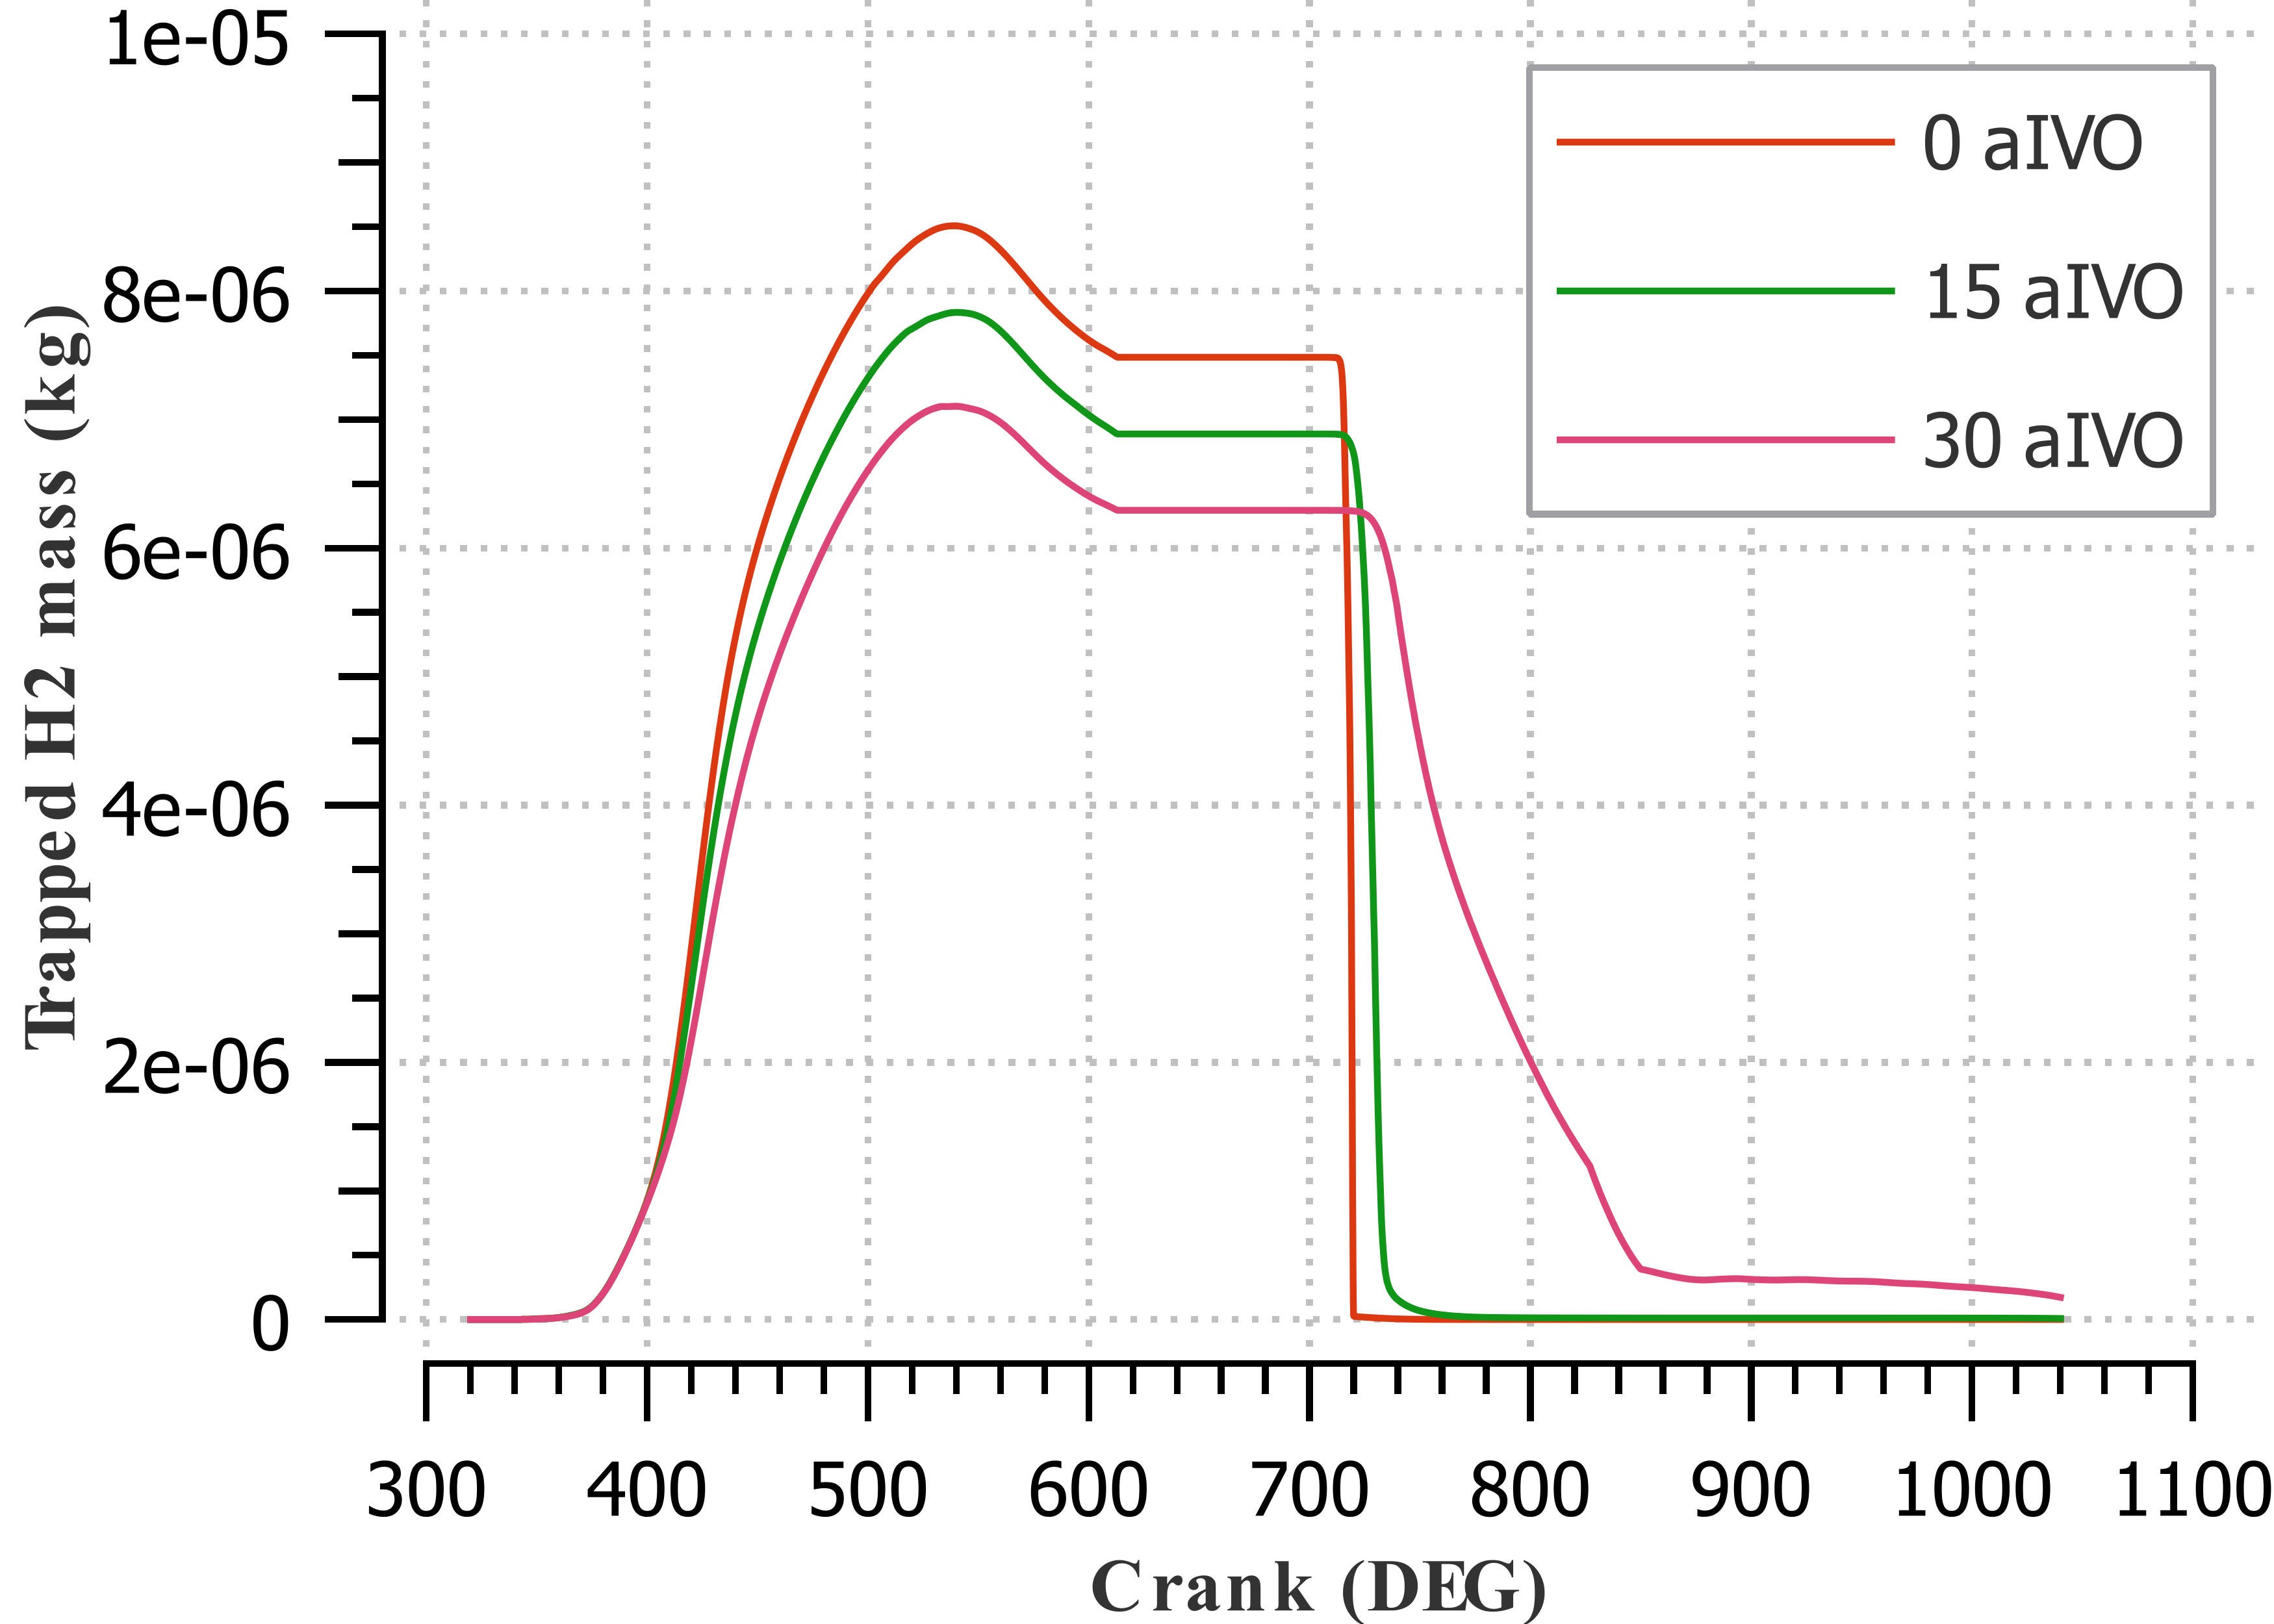
\includegraphics[width=88.9mm]{Plots/30_h2.png}}
    \caption{Trapped Mass for VOT = 30}
    \label{plt_ttt}
    \end{figure}



\subsection{Combustion Simulations}

\section{Results}
\subsection{Trapped Mass}
As we can see on the graph trapped hydrogen mass reduces with delaying injection delay. In the early injection, the injected hydrogen of per cycle can fully flow into the cylinder rapidly. But delayed injection time, the hydrogen gas injected per cycle could not fully enter the cylinder. 

\begin{figure}[htbp]
    \centerline{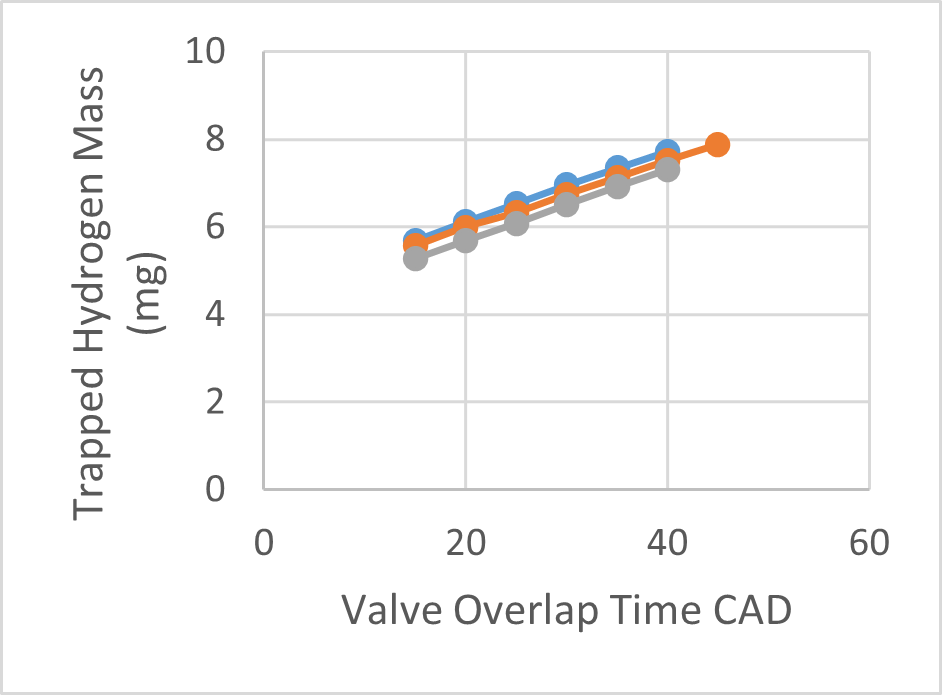
\includegraphics{Plots/trapped mass.png}}
    \caption{Trapped Hydrogen Mass}
    \label{plt_1}
    \end{figure}

\subsection{In-Cylinder Pressure}
\begin{figure}[htbp]
    \centerline{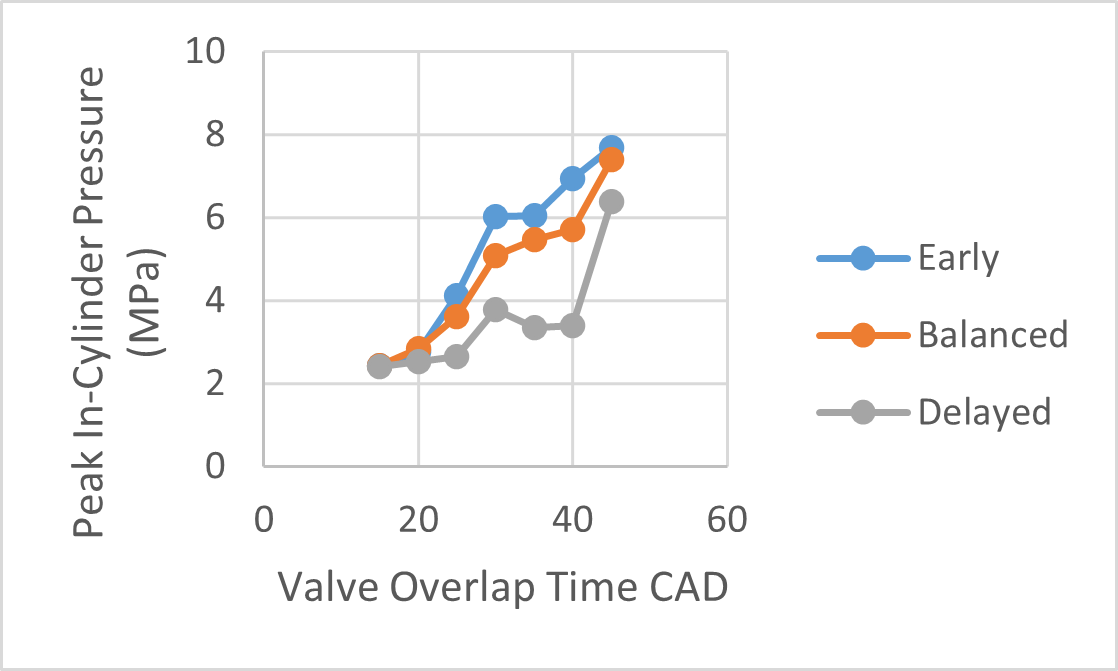
\includegraphics{Plots/pressure.png}}
    \caption{Pressure}
    \label{plt_2}
    \end{figure}

\subsection{In-Cylinder Temperature}
\begin{figure}[htbp]
    \centerline{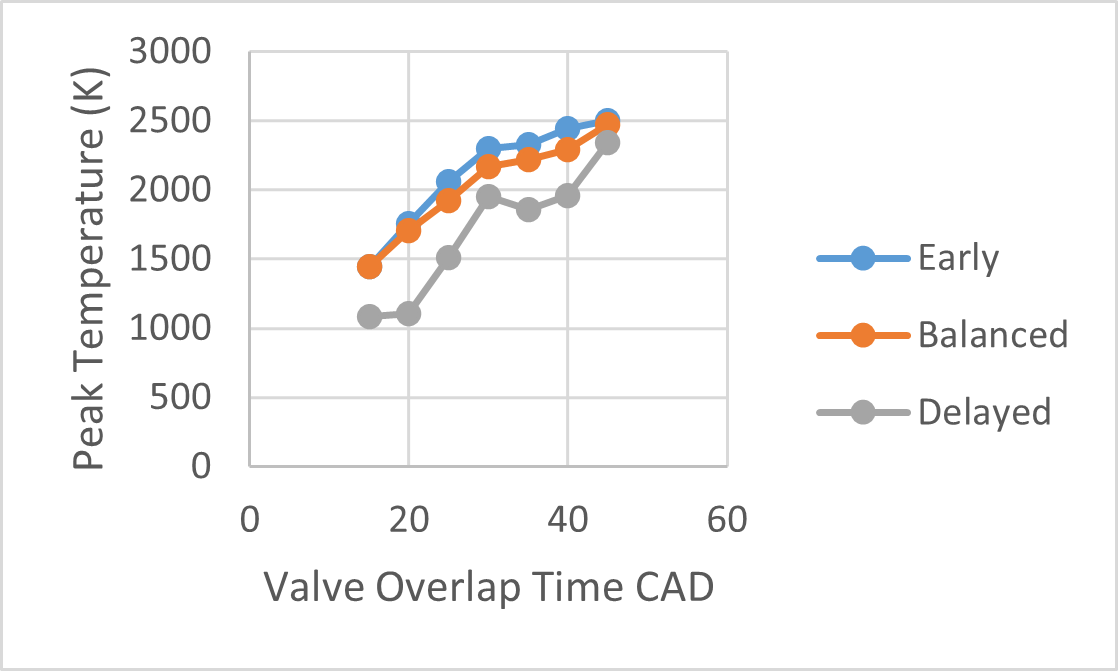
\includegraphics{Plots/temperature.png}}
    \caption{Temperature}
    \label{plt_3}
    \end{figure}

\subsection{Peak Heat Release Rate}
\begin{figure}[htbp]
    \centerline{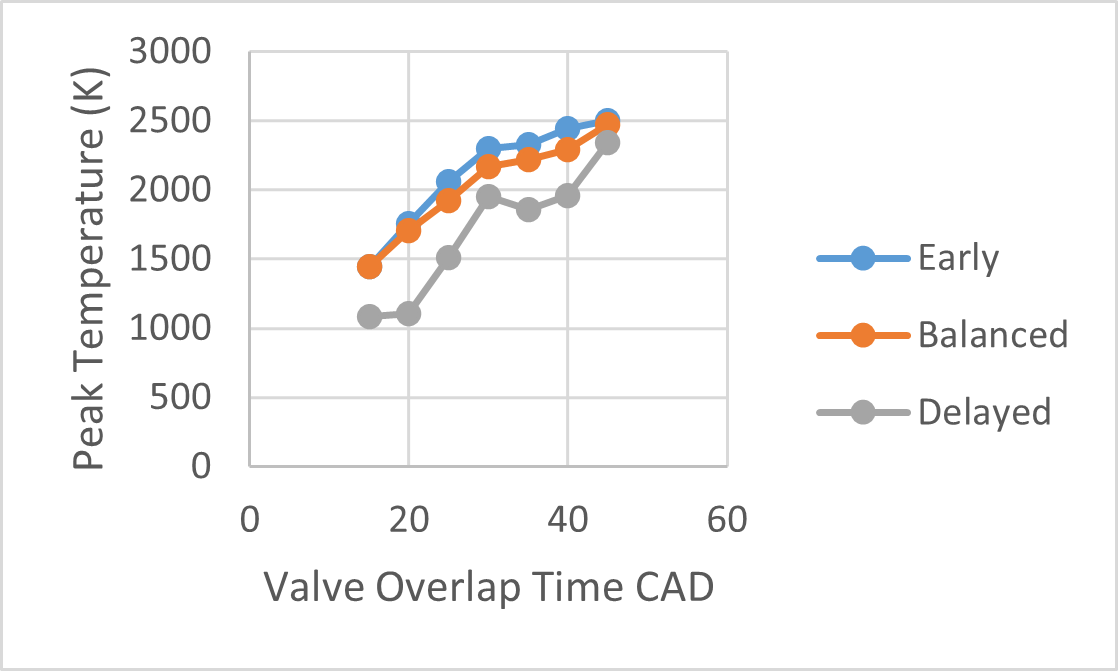
\includegraphics{Plots/hrr.png}}
    \caption{HRR}
    \label{plt_4}
    \end{figure}

Low heat release rate indicates slower rate of chemical reaction while high heat release rate indicates rapid combustion. To produce more useful work from the combustion process, gradual combustion process should be ensured. 
HRR < x can be defined as incomplete combustion and HRR > y can be defined as knocking combustion. Both of which should be eliminated for an effective combustion process.
according to the results, xxxx cases can be defined as inefficient combustion cases.
This rapid burning is due to increased trapped mass within the cylinder and consequently increased equivalence ratios.
Ranges of valve and injection timing for proper combustion characteristics.

\subsection{IMEP}

\subsection{Peak Heat Release Rate}
\begin{figure}[htbp]
    \centerline{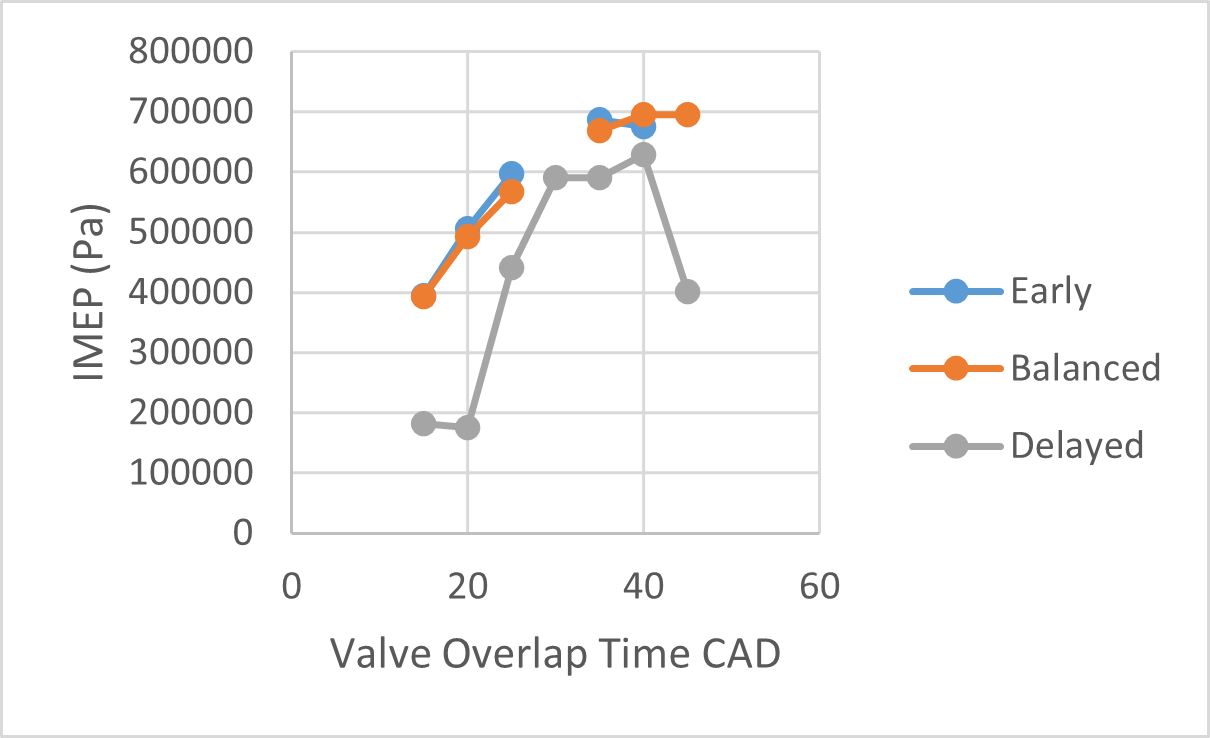
\includegraphics{Plots/imep.png}}
    \caption{IMEP}
    \label{plt_5}
    \end{figure}
Variation of IMEP with VOT and injection mode.
Reduced trapped mass – less time to go to cylinder.
    
\subsection{Efficiency}
\begin{figure}[htbp]
    \centerline{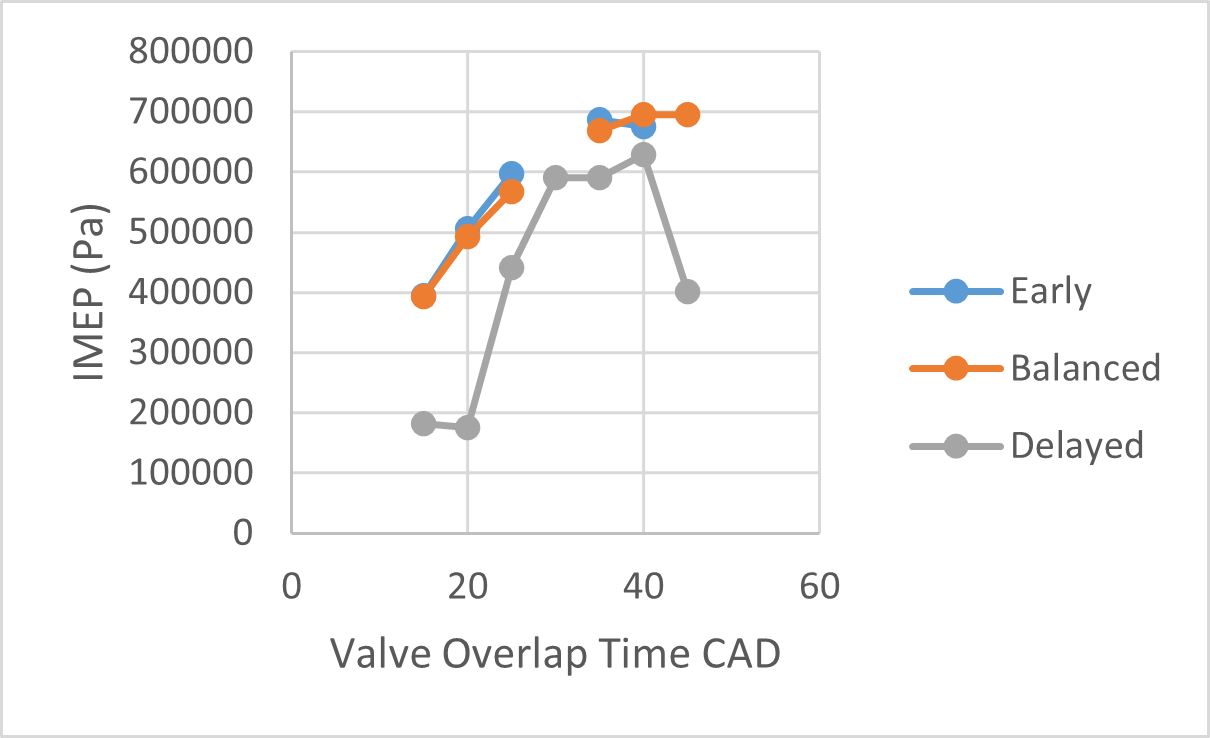
\includegraphics{Plots/imep.png}}
    \caption{Efficiency}
    \label{plt_6}
    \end{figure}
\subsection{Local Concentration}
\begin{figure}[htbp]
    \centerline{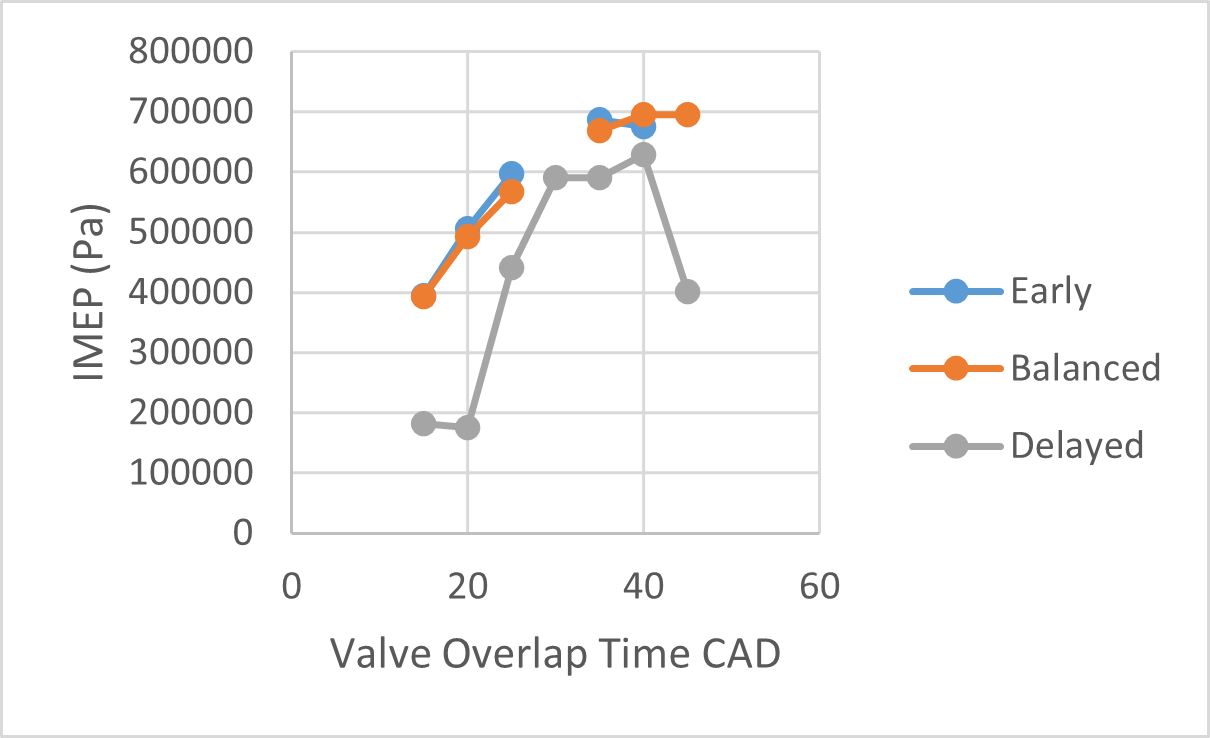
\includegraphics{Plots/imep.png}}
    \caption{Local Concentration}
    \label{plt_7}
    \end{figure}

\section{Conclusion}

\section{Future Works}
Effect of valve and injection timing on backfire, in particular, flame propagation.

\section*{Acknowledgment}



\begin{thebibliography}{00}
\bibitem{b1} L. Wang et al., “The effect of hydrogen injection parameters on the quality of hydrogen–air mixture formation for a PFI hydrogen internal combustion engine,” Int. J. Hydrog. Energy, vol. 42, no. 37, pp. 23832–23845, Sep. 2017, doi: 10.1016/j.ijhydene.2017.04.086.
\bibitem{b2} H. Yun, Z. Bu, Z. Yang, L. Wang, and B. Zhang, “Optimization of fuel injection timing and ignition timing of hydrogen fueled SI engine based on DOE-MPGA,” Int. J. Hydrog. Energy, vol. 48, no. 25, pp. 9462–9473, Mar. 2023, doi: 10.1016/j.ijhydene.2022.12.068.
\bibitem{b3} J. Duan, F. Liu, and B. Sun, “Backfire control and power enhancement of a hydrogen internal combustion engine,” Int. J. Hydrog. Energy, vol. 39, no. 9, pp. 4581–4589, Mar. 2014, doi: 10.1016/j.ijhydene.2013.12.175.
\bibitem{b4} X. Liu, F. Liu, L. Zhou, B. Sun, and H. Schock, “Backfire prediction in a manifold injection hydrogen internal combustion engine,” Int. J. Hydrog. Energy, vol. 33, no. 14, pp. 3847–3855, Jul. 2008, doi: 10.1016/j.ijhydene.2008.04.051.
\bibitem{b5} A. Menaa, M. S. Lounici, F. Amrouche, K. Loubar, and M. Kessal, “CFD analysis of hydrogen injection pressure and valve profile law effects on backfire and pre-ignition phenomena in hydrogen-diesel dual fuel engine,” Int. J. Hydrog. Energy, vol. 44, no. 18, pp. 9408–9422, Apr. 2019, doi: 10.1016/j.ijhydene.2019.02.123.
\bibitem{b6} C. Park, W. Park, Y. Kim, Y. Choi, and B. Lim, “Effect of Valve Timing and Excess Air Ratio on Torque in Hydrogen-Fueled Internal Combustion Engine for UAV,” Energies, vol. 12, no. 5, p. 771, Feb. 2019, doi: 10.3390/en12050771.
\bibitem{b7} T. C. Huynh, J. K. Kang, K. C. Noh, J. T. Lee, and J. A. Caton, “Controlling Backfire Using Changes of the Valve Overlap Period for a Hydrogen-Fueled Engine Using an External Mixture,” in ASME 2007 Internal Combustion Engine Division Fall Technical Conference, Charleston, South Carolina, USA: ASMEDC, Jan. 2007, pp. 243–251. doi: 10.1115/ICEF2007-1702.
\bibitem{b8} J. Lee, K. Lee, J. Lee, and B. Anh, “High power performance with zero NOx emission in a hydrogen-fueled spark ignition engine by valve timing and lean boosting,” Fuel, vol. 128, pp. 381–389, Jul. 2014, doi: 10.1016/j.fuel.2014.03.010.
\bibitem{b9} M. Ó Conaire, H. J. Curran, J. M. Simmie, W. J. Pitz, and C. K. Westbrook, “A comprehensive modeling study of hydrogen oxidation,” Int. J. Chem. Kinet., vol. 36, no. 11, pp. 603–622, Nov. 2004, doi: 10.1002/kin.20036.
\bibitem{10} V. Dhyani and K. A. Subramanian, “Fundamental characterization of backfire in a hydrogen fuelled spark ignition engine using CFD and experiments,” Int. J. Hydrog. Energy, vol. 44, no. 60, pp. 32254–32270, Dec. 2019, doi: 10.1016/j.ijhydene.2019.10.077.

\end{thebibliography}

\end{document}
